
We present following facts according business processes from  Subsection~\ref{sub:ml1_processes}.
\begin{itemize}
    \item Advertisement - poin of view: Added at the end of a day. For each advertisement it would contain sum up information from the whole day.
    \item Subscriptions - point of view: Represent one subscription from one customer.
    \item Article popularity - point of view: Every day we store
    actual information how our articles are popular for every single article.
\end{itemize}

\begin{figure}[!hbp]
\begin{center}
  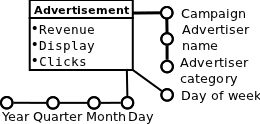
\includegraphics[scale=0.5]{fact_advertisement}
\caption{\label{pic:f_adv}  Advertisement}
\end{center}
\end{figure}

\begin{figure}[!hbp]
\begin{center}
    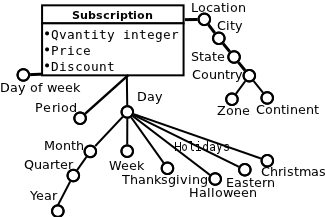
\includegraphics[scale=0.5]{fact_subscriptions}
\caption{\label{pic:f_sub}  Subscriptions}
\end{center}
\end{figure}

\begin{figure}[!hbp]
\begin{center}
  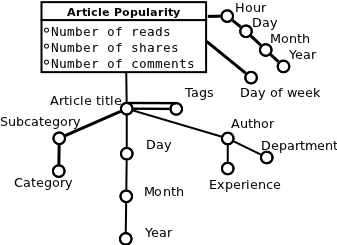
\includegraphics[scale=0.5]{fact_article}
\caption{\label{pic:f_art}  Article popularity}
\end{center}
\end{figure}

